\documentclass[10pt,a4paper]{article}

\usepackage[utf8]{inputenc}
\usepackage[T1]{fontenc}
\usepackage{amsmath,amssymb,amsfonts}
\usepackage{graphicx}
\usepackage{hyperref}
\usepackage{algorithm}
\usepackage{algpseudocode}
\usepackage{geometry}
\usepackage{cite}

% Page layout
\geometry{margin=1.5cm}

% Title page
\title{\Large\textbf{PixelBytes: Catching Unified Embedding for Multimodal Generation}}
\author{\large Fabien Furfaro}
\date{\large 2024}

\begin{document}

\maketitle

\begin{abstract}
This report introduces PixelBytes, a multimodal embedding model designed for generating text and pixelated images simultaneously. We present the PxByEmbed algorithm, which facilitates the efficient representation of mixed sequences. Our approach utilizes web-scraped Pokémon data, image processing techniques, and machine learning methods to create a specialized dataset and training pipeline. The dataset balances text and pixelated images, ensuring an equilibrium in token representation. We constructed it by scraping data from Pokepedia, applying pixelation using OpenCV and scikit-image, and quantizing images with a NES-inspired color palette. We evaluate various model architectures, including Recurrent Neural Networks (RNNs), Transformers, and Mamba models, using metrics such as Hamming distance, cosine similarity, and BLEU scores. Initial results suggest that bidirectional RNN models with PxBy embedding and convolutional layers perform well in generating coherent sequences. Our findings also indicate that compact models can be effective, challenging the assumption that larger models are always superior. Additionally, we observe robustness to input size variations and potential benefits from increased model depth. These insights contribute to the ongoing exploration of model architecture design and the trade-offs between complexity and performance in multimodal generation tasks.
\end{abstract}

\begin{figure}[h]
\centering
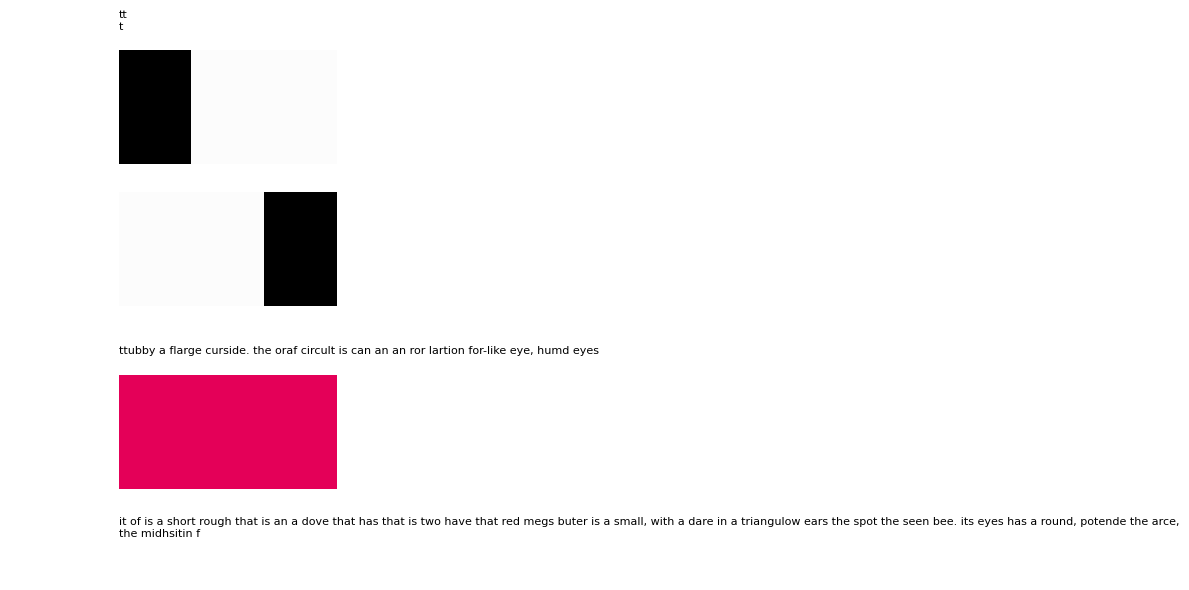
\includegraphics[width=0.8\linewidth]{example_generation.png}
\caption{Example of a generated pixelated Pokémon and its description}
\label{fig:example_generation}
\end{figure}

\section{Introduction}

Multimodal sequence generation, combining diverse data types such as text and numerical sequences, presents a significant challenge in artificial intelligence \cite{baltrusaitis2019multimodal}. While models like GPT have excelled in text generation \cite{brown2020language}, there's a growing need for unified approaches that can seamlessly handle varied data types. Building upon these findings, PixelBytes aims to address the challenge of unified text and image generation by proposing a model capable of producing mixed sequences of text and images in a coherent and unified manner. We draw inspiration from state-of-the-art sequence models, including Image Transformers \cite{parmar2018image}, and recent developments in bidirectional architectures \cite{schuster1997bidirectional, bimamba} and embedding techniques \cite{mikolov2013efficient, mambabyte}. We explore various architectures including Recurrent Neural Networks (RNNs), State Space Models (SSMs), and Attention-based models, focusing on:

\begin{itemize}
    \item The effectiveness of bidirectional processing
    \item Novel embedding techniques, particularly PxBy embedding
    \item The impact of convolutional layers
    \item Effects of model depth, input dimensionality, and model size
\end{itemize}

Our experiments reveal that compact bidirectional RNN models with PxBy embedding and convolutional layers demonstrate superior performance in generating coherent sequences. This finding challenges the notion that larger models are always better, aligning with recent research on model efficiency \cite{tan2019efficientnet}. We evaluate our models using Hamming distance, cosine similarity, and BLEU scores, providing a comprehensive assessment of sequence similarity and quality \cite{papineni2002bleu}. Our results show robustness to input size variations and highlight the benefits of increased model depth in certain scenarios. This paper presents our methodology, experimental results, and analysis, contributing to the development of more effective and versatile sequence generation models.

\section{Model Architecture}

\subsection{Overview}
PixelBytes integrates several innovative components to achieve its multimodal generation capabilities:
\begin{itemize}
    \item A tokenizer sequence constructor for pixelated images and byte-level text representation
    \item A unified multimodal embedding (PxByEmbed)
    \item A bidirectional RNN with convolutional layers for sequence processing
\end{itemize}

This architecture is inspired by recent advancements in multimodal learning \cite{baltrusaitis2019multimodal} and efficient sequence modeling \cite{vaswani2017attention}.

\subsection{Dataset Construction}

Existing image-captioning datasets often prove unsuitable for combined text and image generation due to limited text content and difficulties in interpreting pixelated versions of high-resolution images. To address this, we developed a specialized dataset based on Pokémon data, offering advantages such as a long-standing franchise history, availability of pixelated designs, rich descriptive text, and a diverse collection of over 1000 unique Pokémon. This approach aligns with recent trends in creating specialized datasets for multimodal learning tasks \cite{lin2014microsoft}.

We constructed our dataset by web scraping miniatures and descriptions from Pokepedia using Beautiful Soup \cite{richardson2007beautiful}. The scraped images were then pixelated using OpenCV and scikit-image libraries \cite{bradski2000opencv, vanderwalt2014scikit} to create a retro aesthetic. We maintained a 2/3 text to 1/3 image ratio in the dataset to ensure comprehensive training on both modalities.

For image quantization, we used a palette inspired by the NES color scheme (55 colors), creating tokens that represent different color and position combinations. This approach effectively translates visual information into a format suitable for sequence modeling, similar to recent work in discrete representation learning for images \cite{van2017neural}. The quantization process was implemented using OpenCV and scikit-image, with the NES palette sourced from web-based color palette resources. To ensure a balanced representation, we carefully adjusted the number of image and text tokens, resulting in a total of 113 characters for each modality. This equilibrium allows the model to learn equally from both visual and textual information during training.

The final dataset, balancing text and pixelated images, was uploaded to the Hugging Face Datasets Hub for easy access and reproducibility.

\section{Multimodal Embedding Algorithm}

\subsection{PxByEmbed: Multimodal Embedding Algorithm}

At the core of our approach is the PxByEmbed algorithm, which represents mixed sequences of text and images in a unified manner. This algorithm extends classical embedding techniques by incorporating spatial adaptivity, allowing for more effective representation of both textual and visual information. PxByEmbed builds upon recent advancements in multimodal embeddings \cite{kiela2018learning} and adapts them for the specific needs of pixel-level image representation and byte-level text encoding. The algorithm employs a learned embedding matrix that maps each token (whether text or image) to a high-dimensional vector space, while preserving spatial relationships for image tokens.

\begin{algorithm}[h]
\caption{PxByEmbed: Multimodal Embedding Algorithm (k=3)
\newline
\textbf{Input:} $V$: vocabulary size, $D$: embedding dimension
\newline
\textbf{Output:} Embedded representation $\mathbf{E} \in \mathbb{R}^{B \times L \times D}$
\newline
\textbf{Note:} $\mathbf{X}_{emb} \in \mathbb{R}^{B \cdot L \times E_{int} \times k \times k}$, 
$\mathbf{X}_{flat} \in \mathbb{R}^{B \cdot L \times E_{int}k^2}$, 
$\mathbf{X}_{proj} \in \mathbb{R}^{B \cdot L \times D}$
}
\begin{algorithmic}[0]
\State \textbf{Initialize:}
\State $k \gets 3$
\State $E_{int} \gets \max(9, \lfloor D / k^2 \rfloor)$
\State $\mathbf{\alpha} \in \mathbb{R}^{1 \times 1 \times k \times k}$ 
\State $\mathbf{W}_{emb} \in \mathbb{R}^{V \times E_{int}}$ 
\State $\mathbf{W}_{proj} \in \mathbb{R}^{E_{int}k^2 \times D}$ 
\State $\mathbf{W}_{patch} \in \mathbb{R}^{E_{int} \times E_{int} \times k \times k}$ 

\Function{PxByEmbed}{$\mathbf{X} \in \mathbb{Z}^{B \times L \times k \times k}$}
    \State $\mathbf{X}_{emb} \gets \text{Permute}(\text{Embed}(\mathbf{X}, \mathbf{W}_{emb}), [0, 3, 1, 2])$ 
    
    \State $\mathbf{X}_{patch} \gets \text{Conv2D}(\mathbf{X}_{emb}, \mathbf{W}_{patch}, \text{padding}=1)$
    \State $\mathbf{X}_{combined} \gets \sigma(\mathbf{\alpha}) \odot \mathbf{X}_{emb} + (1 - \sigma(\mathbf{\alpha})) \odot \mathbf{X}_{patch}$
    
    \State $\mathbf{X}_{flat} \gets \text{Flatten}(\mathbf{X}_{combined})$ 
    \State $\mathbf{X}_{proj} \gets \mathbf{X}_{flat}\mathbf{W}_{proj}$ 
    \State $\mathbf{E} \gets \text{LayerNorm}(\mathbf{X}_{proj})$
    \State $\mathbf{E} \gets \text{Reshape}(\mathbf{E}, [B, L, D])$
    \State \Return $\mathbf{E}$
\EndFunction
\end{algorithmic}
\end{algorithm}

\subsection{Managing Transitions}

PixelBytes employs a refined approach to manage transitions between text and image tokens, ensuring coherence during mixed sequence generation. This strategy is applied in both dataset construction and sequence generation.

In the dataset construction phase, we utilize a 2D input sequence method that creates a context window around each token. This method features a configurable 3x3 context window, special separator tokens for modality transitions, and padding to maintain consistent context sizes. Additionally, future tokens are masked to introduce time asymmetry. The \texttt{input\_seq\_construct} function implements these strategies by padding the input array and generating a 3D array where each slice represents the context of a token. This enables the model to learn spatial relationships, which is vital for maintaining coherence in mixed sequences.

During sequence generation, transitions are managed dynamically through the \texttt{\_process\_token} function. This function differentiates between text tokens (bytes) and image tokens (tuples) while handling newline (\texttt{\textbackslash n}) and tab (\texttt{\textbackslash t}) characters for line breaks and indentation. It also maintains a \texttt{sequence\_clock} to track progression and manage transitions. Each new token's context is represented in a 3x3 matrix, informing the model of its position relative to surrounding tokens.

This dynamic approach allows PixelBytes to maintain coherence when transitioning between text and image modalities, ensuring that generated sequences respect the structural integrity of both text and pixel-based images.


\section{Training and Evaluation}

\subsection{Model Architectures}
We implemented and compared three different model architectures: Recurrent Neural Network (RNN), specifically using bidirectional Long Short-Term Memory (LSTM) units \cite{hochreiter1997long}, Transformer \cite{vaswani2017attention}, and Mamba, which is based on the State Space Model (SSM) \cite{gu2022efficiently}. Each architecture was tailored to effectively process our multimodal dataset, which combines pixel data and bytecode sequences from NES games.

\subsection{Training Process}
Training was conducted on dual T4 GPUs from Kaggle, which facilitated the experimentation with these advanced architectures and our large multimodal dataset. The training regime employed various hyperparameters, including a batch size of 32, a learning rate of 0.001, and a total of 200 epochs, with evaluations performed every 5 epochs.

\begin{figure}[htbp]
\centering
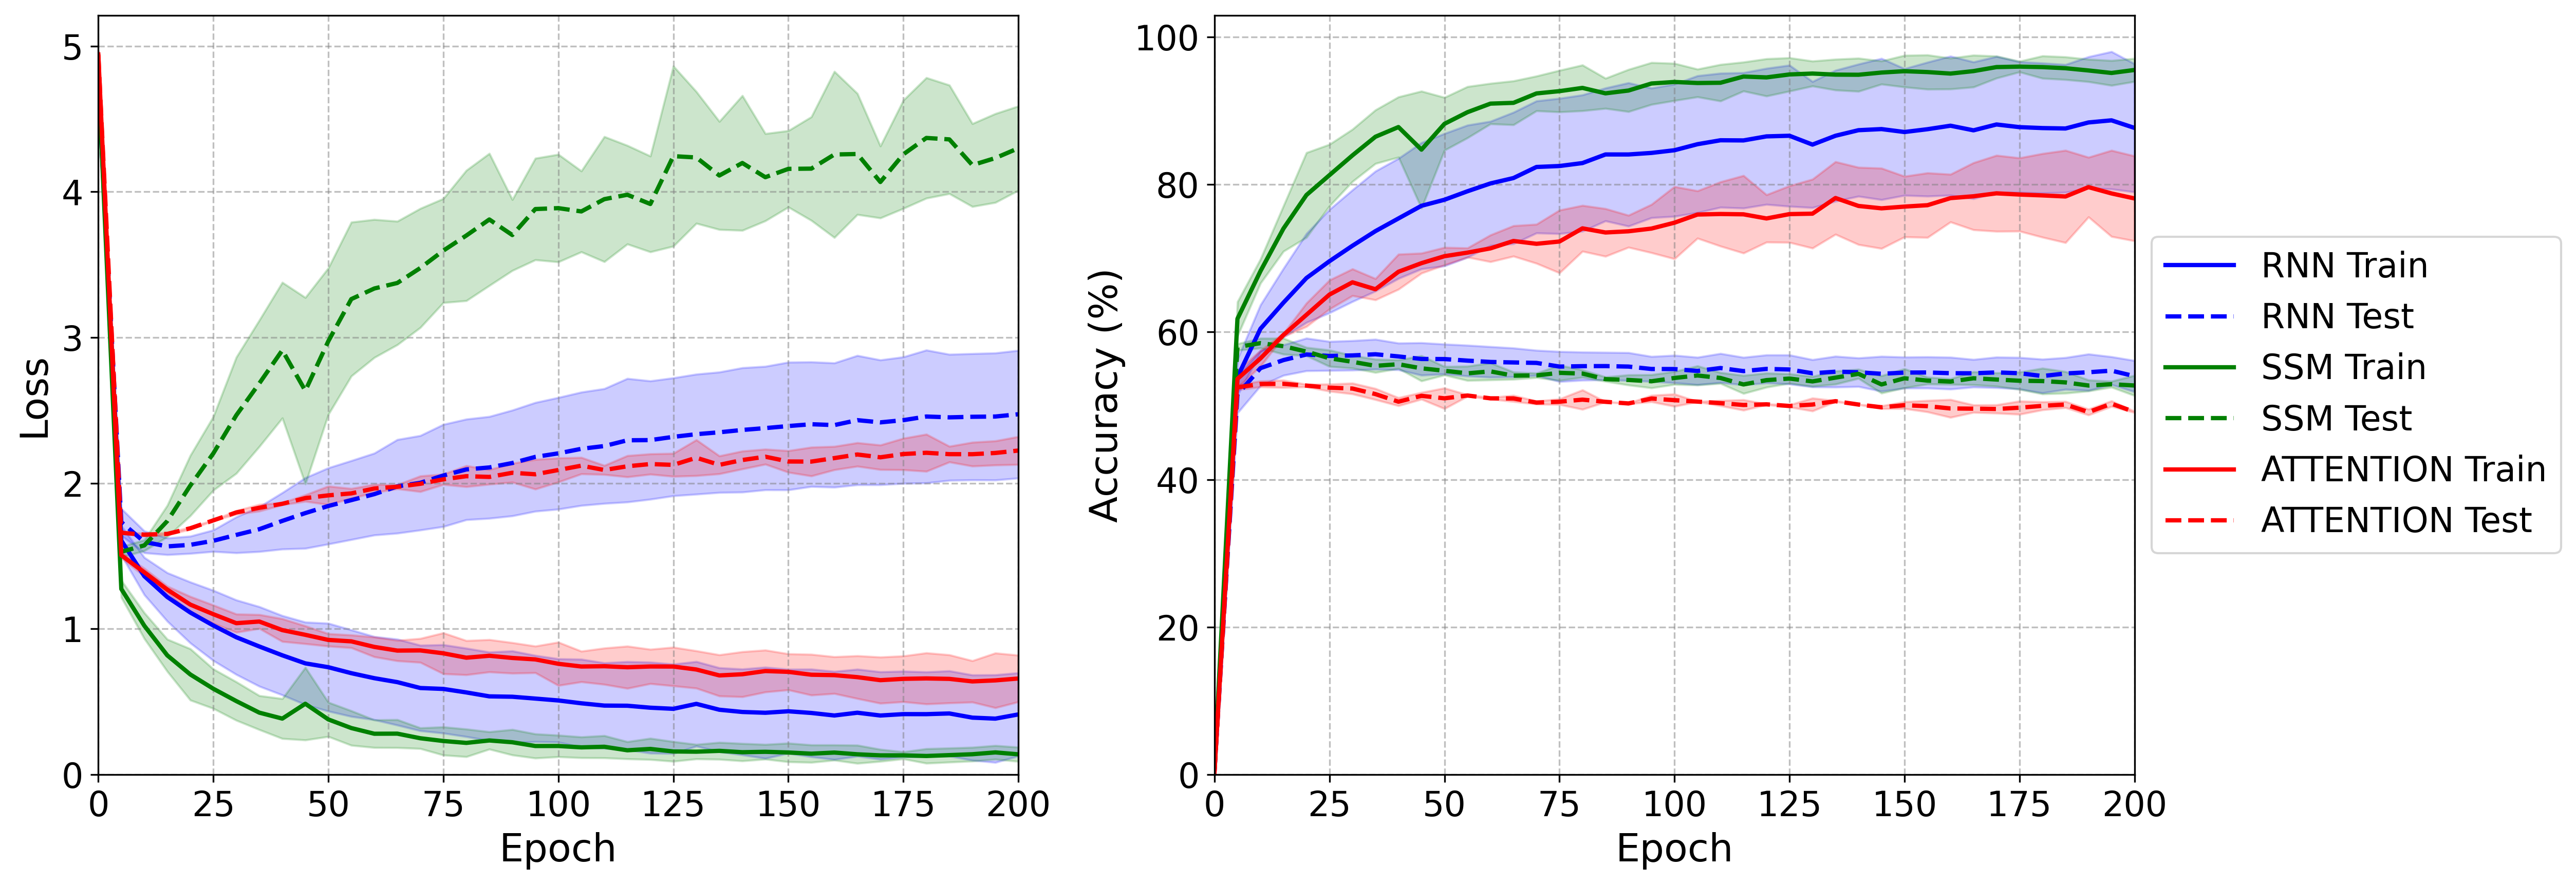
\includegraphics[width=\textwidth]{training_results.png}
\caption{Training and validation metrics (Loss, Accuracy, and F1 Score) for RNN, Transformer, and SSM models over 200 epochs.}
\label{fig:training_results}
\end{figure}

Figure \ref{fig:training_results} illustrates the training and validation metrics for our three model architectures over the course of 200 epochs. The results reveal distinct performance patterns across the different architectures. The State Space Models (SSM) achieved the best training scores in terms of loss, accuracy, and F1 score. However, as evident from the widening gap between training and validation curves, they exhibited signs of overfitting over the epochs. This suggests that while SSMs quickly learned to fit the training data, they struggled to generalize to unseen examples.

In contrast, the LSTMs, denoted as RNNs in our analysis, demonstrated more balanced performance. The closer alignment of their training and validation curves indicates a better compromise between model capacity and generalization capabilities. This robustness makes RNNs a strong candidate for our task of NES game data processing and generation. Interestingly, the Transformer architecture yielded the lowest performance metrics among the three models. This outcome is noteworthy and should be contextualized, as our implementation did not incorporate positional encoding, which is crucial for the effective functioning of transformer models in sequence tasks. The relatively poor performance of the Transformer model underscores the importance of architecture-specific optimizations in sequence modeling tasks.

Overall, these results highlight the trade-offs between different architectures and the importance of careful model selection and tuning for our specific task. While SSMs showed impressive training performance, their tendency to overfit suggests that additional regularization techniques might be necessary for optimal performance. The stable performance of RNNs across both training and validation sets indicates their suitability for this particular task, balancing good fit and generalization.

\subsection{Generation Evaluation Metrics}

Our experiments utilize various model architectures including State Space Models (SSM), Attention models (Att), and Recurrent Neural Networks (RNN) for generating 16 consecutive sequences. We employ three key metrics as described by \cite{sutskever2014sequence}, \cite{hamming1950error}, and \cite{papineni2002bleu}:

\begin{itemize}
    \item \textbf{Hamming Distance}: Scaled 0-1, lower values indicate greater similarity.
    \item \textbf{Cosine Similarity}: Ranges -1 to 1, higher values suggest greater similarity.
    \item \textbf{BLEU Score}: Varies 0-1, higher scores indicate better quality.
\end{itemize}

\begin{table}[h]
\centering
\small
\begin{tabular}{cccccccccc}
\hline
Type & Dir. & Emb. & Conv. & In & Mod & Depth & Hamming & Cosine & BLEU \\
\hline
SSM & Bi & PxBy & Y & 81 & 64 & 1 & 0.170 $\pm$ 0.086 & 0.883 $\pm$ 0.105 & 0.753 $\pm$ 0.115 \\
SSM & Bi & PxBy & Y & 81 & 64 & 2 & 0.158 $\pm$ 0.074 & 0.896 $\pm$ 0.095 & 0.771 $\pm$ 0.097 \\
SSM & Uni & PxBy & Y & 81 & 64 & 2 & 0.166 $\pm$ 0.081 & 0.886 $\pm$ 0.102 & 0.760 $\pm$ 0.106 \\
Att & Bi & PxBy & Y & 81 & 64 & 1 & 0.157 $\pm$ 0.064 & 0.887 $\pm$ 0.103 & 0.765 $\pm$ 0.088 \\
Att & Bi & PxBy & Y & 81 & 64 & 2 & 0.159 $\pm$ 0.066 & 0.887 $\pm$ 0.103 & 0.760 $\pm$ 0.092 \\
RNN & Bi & Center & Y & 81 & 64 & 2 & 0.185 $\pm$ 0.074 & 0.888 $\pm$ 0.083 & 0.750 $\pm$ 0.093 \\
RNN & Bi & PxBy & N & 81 & 64 & 2 & 0.153 $\pm$ 0.061 & 0.902 $\pm$ 0.090 & 0.777 $\pm$ 0.083 \\
RNN & Bi & PxBy & Y & 162 & 64 & 2 & 0.152 $\pm$ 0.062 & 0.905 $\pm$ 0.089 & 0.778 $\pm$ 0.084 \\
RNN & Bi & PxBy & Y & 36 & 64 & 2 & 0.152 $\pm$ 0.061 & 0.904 $\pm$ 0.090 & 0.778 $\pm$ 0.083 \\
RNN & Bi & PxBy & Y & 81 & 128 & 2 & 0.153 $\pm$ 0.063 & 0.903 $\pm$ 0.091 & 0.776 $\pm$ 0.086 \\
RNN & Bi & PxBy & Y & 81 & 32 & 2 & \textbf{0.149} $\pm$ 0.062 & 0.899 $\pm$ 0.095 & \textbf{0.785} $\pm$ 0.082 \\
RNN & Bi & PxBy & Y & 81 & 64 & 1 & 0.149 $\pm$ 0.062 & 0.897 $\pm$ 0.096 & 0.780 $\pm$ 0.085 \\
RNN & Bi & PxBy & Y & 81 & 64 & 3 & 0.153 $\pm$ 0.063 & \textbf{0.906} $\pm$ 0.087 & 0.776 $\pm$ 0.086 \\
RNN & Bi & PxBy & N & 81 & 64 & 2 & 0.151 $\pm$ 0.062 & 0.903 $\pm$ 0.090 & 0.779 $\pm$ 0.084 \\
RNN & Uni & PxBy & Y & 81 & 64 & 2 & 0.153 $\pm$ 0.064 & 0.904 $\pm$ 0.088 & 0.777 $\pm$ 0.087 \\
\hline
\end{tabular}
\caption{Comparison of model characteristics and performance (mean $\pm$ std)}
\label{tab:model_comparison}
\end{table}

The results reveal interesting patterns across different model architectures. SSM models show competitive performance, with the bidirectional 2-layer model achieving better results than its unidirectional counterpart. Attention models demonstrate consistent performance across depths, with slight improvements in the 1-layer model. RNN models, particularly those with PxBy embedding, consistently outperform other architectures. The best Hamming distance (0.149 $\pm$ 0.062) and BLEU score (0.785 $\pm$ 0.082) are achieved by the bidirectional PxBy RNN model with convolution, 81 input dimensions, and 32 model dimensions. This suggests that a more compact RNN model can effectively capture sequence patterns, aligning with findings on model compression \cite{han2016deep}.

The highest cosine similarity (0.906 $\pm$ 0.087) is obtained by the 3-layer RNN model, indicating that increased depth can enhance sequence alignment \cite{pascanu2014construct}. Convolution generally improves performance in RNN models, supporting \cite{lecun1995convolutional}'s findings on local pattern capture. Interestingly, varying the input dimension (36, 81, 162) in RNN models had minimal impact on performance, suggesting robustness to input size changes. The center embedding in RNNs showed lower performance compared to PxBy embedding, highlighting the effectiveness of the latter for this task.

\section{Results and Discussion}

Our experiments with various model architectures and configurations yielded significant findings for the task of NES game data processing and generation. We evaluated the performance of the models based on several metrics, including Hamming distance, cosine similarity, and BLEU score \cite{papineni2002bleu}.

\subsection{Model Performance}

The bidirectional RNN models, particularly those utilizing PixelBytes (PxBy) embedding with convolutional layers, consistently outperformed other architectures across our evaluation metrics. Key observations include:

\begin{itemize}
    \item \textbf{Embedding Strategy}: The PxBy embedding strategy significantly enhanced model performance. The mean BLEU score improved from 0.750 for the center-only approach to 0.777 for the PxBy embedding, demonstrating the importance of utilizing richer representations of the input data.
    
    \item \textbf{Model Architecture}: Bidirectional models outperformed their unidirectional counterparts. The bidirectional RNN achieved a BLEU score of 0.777, compared to 0.776 for the unidirectional model, suggesting that bidirectionality is crucial for capturing the dependencies in sequential data.
    
    \item \textbf{Model Configuration}: Variations in state dimension and layer count had minimal impact on performance. Models with state dimensions of 32, 64, and 128 achieved BLEU scores of 0.784, 0.777, and 0.775 respectively, indicating that our base configuration was sufficiently expressive for the task.
\end{itemize}

\subsection{Comparative Analysis}

The superior performance of bidirectional PxBy RNN models with convolution for our sequence modeling task is evident. However, the potential of State Space Models (SSM) and Attention models in certain scenarios cannot be overlooked. The SSM models, in particular, exhibited rapid convergence and strong training performance, suggesting their viability for future exploration in multimodal data processing.

These findings contribute to the growing body of research on multimodal sequence modeling \cite{baltrusaitis2019multimodal} and highlight the importance of architecture selection and embedding strategies in processing complex, multimodal data such as video game content.

\section{Conclusion and Future Directions}

This study on PixelBytes opens new avenues in unified multimodal generation, demonstrating promising potential for coherent text-image generation in the context of NES game data. The superior performance of bidirectional RNN models with PxBy embedding underscores the importance of comprehensive spatial information and context in processing game data. Future work will focus on:

\begin{itemize}
    \item Refining the PxByEmbed algorithm to further improve its effectiveness in capturing spatial and temporal relationships in game data.
    \item Exploring larger and more diverse datasets to enhance the generalizability of our models.
    \item Investigating applications in creative content generation, such as level design or narrative creation for retro-style games.
    \item Further optimizing SSM and Attention models to better compete with RNN architectures in this specific domain.
\end{itemize}

These directions aim to build upon our current findings and push the boundaries of multimodal sequence modeling in the context of video game content generation.


\bibliographystyle{plain}
\bibliography{references}

\end{document}
